\section{Population Growth and the Logistic Equation} 
\label{S:7.6.Logistic}

\vspace*{-14 pt}
\framebox{\hspace*{3 pt}
\parbox{\boxwidth}{\begin{goals}
\item How can we use differential equations to realistically model the growth of a
  population? 
\item How can we assess the accuracy of our models?
\end{goals}} \hspace*{3 pt}}

\subsection*{Introduction}

The growth of the earth's population is one of the pressing issues of
our time.  Will the population continue to grow?  Or will it perhaps 
level off at some point, and if so, when?  In this section, we
will look at two ways in which we may use differential equations to
help us address questions such as these.

Before we begin, let's consider again two important differential
equations that we have seen in earlier work this chapter.

\begin{exercises} 
  \item  The logistic equation may be used to model how a rumor spreads
    through a group of people.  Suppose that $p(t)$ is the fraction of
    people that have heard the rumor on day $t$.  The equation
    $$
    \frac{dp}{dt} = 0.2p(1-p)
    $$
    describes how $p$ changes.  Suppose initially that one-tenth of
    the people have heard the rumor; that is, $p(0) = 0.1$.

    \ba
    \item What happens to $p(t)$ after a very long time?

    \item Determine a formula for the function $p(t)$.

    \item At what time is $p$ changing most rapidly?

    \item How long does it take before 80\% of the people have heard
      the rumor?

      \ea

  \item Suppose that $b(t)$ measures the number of bacteria living in
    a colony in a Petri dish, where $b$ is measured in thousands and
    $t$ is measured in days.  One day, you measure that there are
    6,000 bacteria and the per capita growth rate is 3.  A few days
    later, you measure that there are 9,000 bacteria and the per
    capita growth rate is 2.  

    \ba
  \item Assume that the per capita growth rate 
    $\frac{db/dt}{b}$ is a linear function of $b$.  Use the
    measurements to find this function and write a logistic equation
    to describe $\frac{db}{dt}$.

  \item What is the carrying capacity for the bacteria?

  \item At what population is the number of bacteria increasing most
    rapidly?
    
  \item If there are initially 1,000 bacteria, how long will it take
    to reach 80\% of the carrying capacity?

    \ea

  \item 
    Suppose that the population of a species of fish is controlled by
    the logistic equation
    $$
    \frac{dP}{dt} = 0.1P(10 - P),
    $$
    where $P$ is measured in thousands of fish and $t$ is measured in
    years.  

    \ba
    \item What is the carrying capacity of this population?

    \item Suppose that a long time has passed and that the fish
      population is stable at the carrying capacity.  At this time,
      humans begin harvesting 20\% of the fish every year.  Modify the
      differential equation by adding a term to incorporate the
      harvesting of fish.

    \item What is the new carrying capacity?

    \item What will the fish population be one year after the
      harvesting begins?

    \item How long will it take for the population to be within 10\%
      of the carrying capacity?
    \ea

\end{exercises}
\afterexercises




\subsection*{The earth's population}

We will now begin studying the earth's population.  To get started,
here are some data for the earth's population in recent years that we
will use in our investigations.

\begin{center}
  \begin{tabular}{|c|c|}
    \hline
    Year & Population (in billions) \\
    \hline
    1998 & 5.932 \\
    1999 & 6.008 \\
    2000 & 6.084 \\
    2001 & 6.159 \\
    2002 & 6.234 \\
    2005 & 6.456 \\
    2006 & 6.531 \\
    2007 & 6.606 \\
    2008 & 6.681 \\
    2009 & 6.756 \\
    2010 & 6.831 \\
    \hline
  \end{tabular}
\end{center}

\begin{activity} \label{A:7.6.1}  
  Our first model will be based on the following assumption:
  \begin{quote}{\em
      The rate of change of the population is proportional to the
      population.  
    }
  \end{quote}

  On the face of it, this seems pretty reasonable.  When there is a
  relatively small number of people, there will be fewer births and
  deaths so the rate of change will be small.  When there is a larger
  number of people, there will be more births and deaths so we expect
  a larger rate of change.

  If $P(t)$ is the population $t$ years after the year 2000, we may
  express this assumption as
  $$
  \frac{dP}{dt} = kP
  $$
  where $k$ is a constant of proportionality.

\ba
\item Use the data in the table to estimate the derivative $P'(0)$
  using a central difference.  Assume that $t=0$ corresponds to the
  year 2000.

\item What is the population $P(0)$?

\item Use these two facts to estimate the constant of proportionality
  $k$ in the differential equation.

\item Now that we know the value of $k$, we have the initial
  value problem
  $$
    \frac{dP}{dt} = kP, \ P(0) = 6.084.
  $$
  Find the solution to this initial value problem.

\item What does your solution predict for the population in the year
  2010?  Is this close to the actual population given in the table?

\item When does your solution predict that the population will reach
  12 billion?

\item What does your solution predict for the population in the year
  2500? 

\item Do you think this is a reasonable model for the earth's
  population?  Why or why not?  Explain your thinking using a couple
  of complete sentences. 

\ea
\end{activity}
\begin{smallhint}
\ba
	\item Small hints for each of the prompts above.
\ea
\end{smallhint}
\begin{bighint}
\ba
	\item Big hints for each of the prompts above.
\ea
\end{bighint}
\begin{activitySolution}
\ba
	\item Solutions for each of the prompts above.
\ea
\end{activitySolution}
\aftera

Our work in Activity~\ref{A:7.6.1} shows that that the exponential model is fairly accurate for years 
relatively close to 2000.  However, if we go too far into the
future, the model predicts increasingly large rates of change, which
causes the population to grow arbitrarily large.  This does not make
much sense since it is unrealistic to expect that the earth would be able to support
such a large population.  

The constant $k$ in the differential equation has an important
interpretation.  Let's rewrite the differential equation $\frac{dP}{dt} = kP$ by solving for $k$, so that we have
$$k = \frac{dP/dt}{P}.$$
Viewed in this light, $k$ is the ratio of the rate of change to the
population;  in other words, it is the contribution to the rate of change 
from a single person.  We call this the {\em per capita
  growth rate}\index{per capita growth rate}.

In the exponential model we introduced in Activity~\ref{A:7.6.1}, the per capita growth rate is
constant.  In particular, we are assuming that when the population is
large, the per capita growth rate is the same as when the population
is small.  It is natural to think that the per capita growth rate should
decrease when the population becomes large, since there will not be
enough resources to support so many people.  In other words, we expect that a more realistic model would hold if we assume
that the per capita growth rate depends on the population $P$.

In the previous activity, we computed the per capita growth rate in a
single year by computing $k$, the quotient of $\frac{dP}{dt}$ and $P$ (which we did for $t = 0$).  If we return data and compute the per capita
growth rate over a range of years, we generate the data shown in Figure~\ref{F:7.6.census}, which shows how the per capita growth rate is a function of the population, $P$.  
\begin{figure}[h]
\begin{center}
  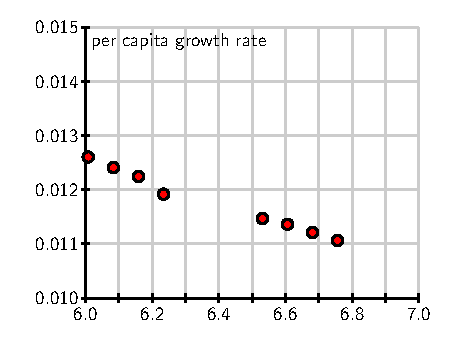
\includegraphics{figures/7_6_census.eps}
\end{center}
\caption{A plot of per capita growth rate vs.~population $P$.} \label{F:7.6.census}
\end{figure}
From the data, we see that the per capita growth rate appears to decrease as
the population increases.  In fact, the points seem to lie very close
to a line, which is shown at two different scales in Figure~\ref{F:7.6.census1}.
\begin{figure}[h]
\begin{center}
  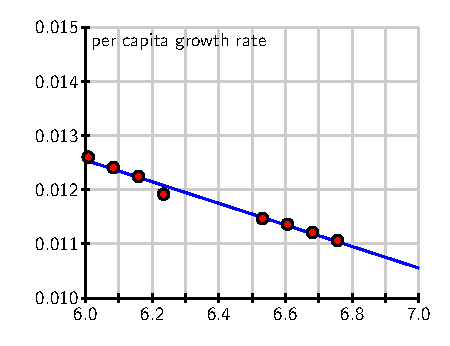
\includegraphics{figures/7_6_census_1.eps} \qquad
  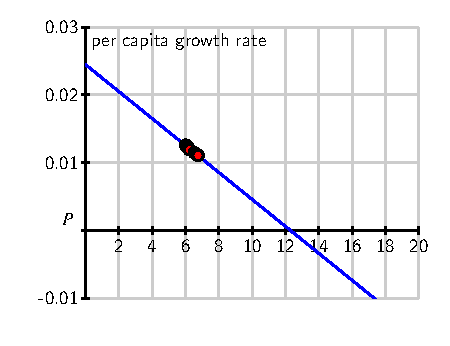
\includegraphics{figures/7_6_census_2.eps} \qquad
\end{center}
\caption{The line that approximates per capita growth as a function of population, $P$.} \label{F:7.6.census1}
\end{figure}
Looking at this line carefully, we can find its equation to be
$$
\frac{dP/dt}{P} = 0.025 - 0.002P.
$$
If we multiply both sides by $P$, we arrive at the differential
equation
$$
\frac{dP}{dt} = P(0.025 - 0.002P).
$$
Graphing the dependence of $dP/dt$ on the population $P$, we see that this differential equation demonstrates a quadratic relationship between $\frac{dP}{dt}$ and $P$, as shown in Figure~\ref{F:7.6.logistic}.
\begin{figure}[h]
\begin{center}
  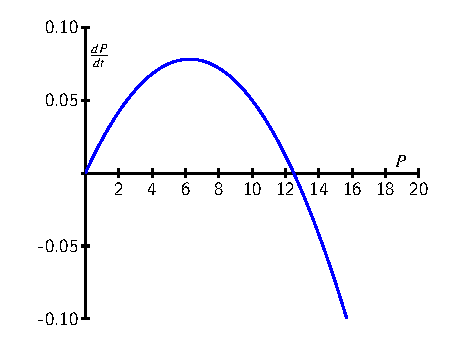
\includegraphics{figures/7_6_logistic_de.eps}
\end{center}
\caption{A plot of $\frac{dP}{dt}$ vs.~$P$ for the differential equation $\frac{dP}{dt} = P(0.025 - 0.002P)$.}\label{F:7.6.logistic}
\end{figure}
The equation $\frac{dP}{dt} = P(0.025 - 0.002P)$ is an example of the {\em logistic equation}, 
and is the second model for population growth that we will consider.  We
have reason to believe that it will be more realistic since the per
capita growth rate is a decreasing function of the population.

Indeed, the graph in Figure~\ref{F:7.6.logistic} shows that there are two equilibrium
solutions, $P=0$, which is unstable, and $P=12.5$, which is a stable
equilibrium.  The graph shows that any solution with $P(0) >0$ will
eventually stabilize around 12.5.  In other words, our model predicts
the world's population will eventually stabilize around 12.5
billion.

A prediction for the long-term behavior of the population is a
valuable conclusion to draw from our differential equation.  We would,
however, like to answer some quantitative questions.  For instance,
how long will it take to reach a population of 10 billion?  To determine this,
we need to find an explicit solution of the equation.  

\subsection*{Solving the logistic differential equation} \index{logistic}

Since we would like to apply the logistic model in more general situations, we state the logistic equation\index{logistic equation} in its more general form,
\begin{equation} \label{E:7.6.logistic}
\frac{dP}{dt} = kP(N-P).
\end{equation}
The equilibrium solutions here are when $P=0$ and $1-\frac PN = 0$,
which shows that $P=N$.  The equilibrium at $P=N$ is called the {\em
  carrying capacity}\index{carrying capacity} of the population for it represents the stable
population that can be sustained by the environment.

We now solve the logistic equation~(\ref{E:7.6.logistic}).  The equation is separable, so we separate the variables
$$
\frac{1}{P(N-P)}\frac{dP}{dt} = k,
$$
and integrate to find that
$$
\int \frac{1}{P(N-P)}~dP = \int k~dt.
$$

To find the antiderivative on the left, we use the partial fraction decomposition
$$
\frac{1}{P(N-P)} = \frac 1N\left[\frac 1P + \frac 1{N-P}\right].
$$
Now we are ready to integrate, with 
$$
\int \frac 1N\left[\frac 1P + \frac 1{N-P}\right] ~dP  =  \int k~dt. 
$$
On the left, observe that $N$ is constant, so we can remove the factor of $\frac{1}{N}$ and antidifferentiate to find that
$$
\frac 1N (\ln|P| - \ln|N-P|)  =  kt + C.
$$
Multiplying both sides of this last equation by $N$ and using an important rule of logarithms, we next find that
$$\ln\left|\frac{P}{N-P}\right| = kNt + C.$$
From the definition of the logarithm, replacing $e^C$ with $C$, and letting $C$ absorb the absolute value signs, we now know that 
$$\frac{P}{N-P} =  Ce^{kNt}.$$
At this point, all that remains is to determine $C$ and solve algebraically for $P$.

If the initial population is $P(0) = P_0$, then it follows that $C = \frac{P_0}{N-P_0}$, so
$$\frac{P}{N-P} = \frac{P_0}{N-P_0}e^{kNt}.$$
We will solve this most recent equation for $P$ by multiplying both sides by
$(N-P)(N-P_0)$ to obtain 
\begin{eqnarray*}
P(N-P_0) &=& P_0(N-P)e^{kNt}  \\
	 &=& P_0Ne^{kNt} - P_0Pe^{kNt}. 
\end{eqnarray*}	 
Swapping the left and right sides, expanding, and factoring, it follows that
\begin{eqnarray*}
P_0Ne^{kNt} & = & P(N-P_0) + P_0 Pe^{kNt}  \\
	& = & P(N-P_0 + P_0e^{kNt}). 
\end{eqnarray*}
Dividing to solve for $P$, we see that
$$P = \frac{P_0Ne^{kNt}}{N-P_0 + P_0e^{kNt}}.$$
Finally, we choose to multiply the numerator and denominator by $\frac{1}{P_0}e^{-kNt}$
to obtain
$$
P(t) = \frac{N}{\left(\frac{N-P_0}{P_0}\right) e^{-kNt} + 1}.
$$

While that was a lot of algebra, notice the result:  we have
found an explicit solution to the initial value problem
$$
  \frac{dP}{dt} = kP(N-P), \ P(0) = P_0,
$$
and that solution\index{logistic equation!solution} is 
\begin{equation}\label{E:7.6.logistic_solution}
P(t) = \frac{N}{\left(\frac{N-P_0}{P_0}\right) e^{-kNt} + 1}.
\end{equation}

For the logistic equation describing the earth's population that we worked with earlier in this section, we have
$$k=0.002, \quad N= 12.5, \quad \hbox{and} \quad P_0 = 6.084.$$
This gives the solution
$$
P(t) = \frac{12.5}{1.0546e^{-0.025t} + 1},
$$
whose graph is shown in Figure~\ref{F:7.6.logistic_sol}
\begin{figure}[h]
\begin{center}
  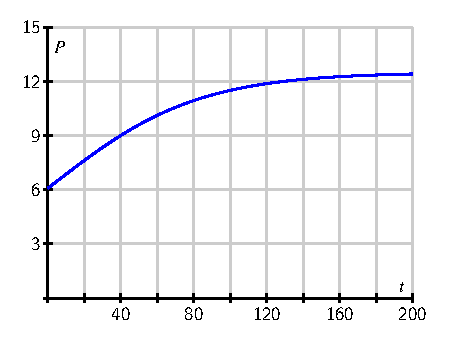
\includegraphics{figures/7_6_logistic_sol.eps}
\end{center}
\caption{The solution to the logistic equation modeling the earth's population.} \label{F:7.6.logistic_sol}
\end{figure}
Notice that the graph shows the population leveling off at 12.5 billion, as
we expected, and that the population will be around 10 billion in the
year 2050.  These results, which we have found using a relatively simple
mathematical model, agree fairly well with predictions made using a
much more sophisticated model developed by the United Nations.

The logistic equation is useful in other situations, too, as it is good for modeling any situation in which limited growth is possible.  For instance, it could model the spread of a flu virus through a population contained on a cruise ship, the rate at which a rumor spreads within a small town, or the behavior of an animal population on an island.  Again, it is important to realize that through our work in this section, we have completely solved the logistic equation, regardless of the values of the constants $N$, $k$, and $P_0$.  Anytime we encounter a logistic equation, we can apply the formula we found in Equation~(\ref{E:7.6.logistic_solution}).

\begin{activity} \label{A:7.6.2}  
  Consider the logistic equation
  $$
  \frac{dP}{dt} = kP(N-P)
  $$
  with the graph of $\frac{dP}{dt}$ vs.~$P$ shown below.
  \begin{center}
    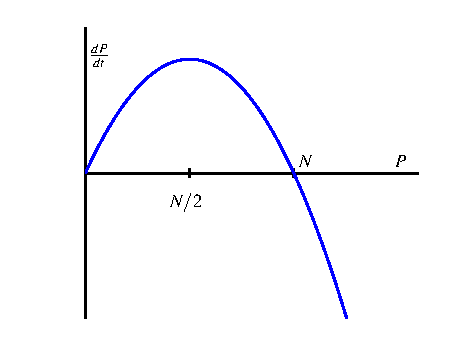
\includegraphics{figures/7_6_activity_2.eps}
  \end{center}
\ba
\item At what value of $P$ is the rate of change greatest?

\item Consider the model for the earth's population that we created.
  At what value of $P$ is the rate of change greatest?  How does that
  compare to the population in recent years?

\item According to the model we developed, what will the population be
  in the year 2100?

\item According to the model we developed, when will the population
  reach 9 billion?

\item Now consider the general solution to the general logistic initial value problem that
  we found, given by
  $$
  P(t) = \frac{N}{\left(\frac{N-P_0}{P_0}\right)e^{-kNt} + 1}.
  $$
  Verify algebraically that $P(0) = P_0$ and that $\lim_{t\to\infty} P(t) = N$.

\ea
\end{activity}
\begin{smallhint}
\ba
	\item Small hints for each of the prompts above.
\ea
\end{smallhint}
\begin{bighint}
\ba
	\item Big hints for each of the prompts above.
\ea
\end{bighint}
\begin{activitySolution}
\ba
	\item Solutions for each of the prompts above.
\ea
\end{activitySolution}
\aftera

\begin{summary}
\item If we assume that the rate of growth of a population is
  proportional to the population, we are led to a model in which the
  population grows without bound and at a  rate that grows without bound. 
\item By assuming that the per capita growth rate decreases as the
  population grows, we are led to the logistic model of population
  growth, which predicts that the population will eventually
  stabilize at the carrying capacity.
\end{summary}

\nin \hrulefill

\begin{exercises} 
  \item  The logistic equation may be used to model how a rumor spreads
    through a group of people.  Suppose that $p(t)$ is the fraction of
    people that have heard the rumor on day $t$.  The equation
    $$
    \frac{dp}{dt} = 0.2p(1-p)
    $$
    describes how $p$ changes.  Suppose initially that one-tenth of
    the people have heard the rumor; that is, $p(0) = 0.1$.

    \ba
    \item What happens to $p(t)$ after a very long time?

    \item Determine a formula for the function $p(t)$.

    \item At what time is $p$ changing most rapidly?

    \item How long does it take before 80\% of the people have heard
      the rumor?

      \ea

  \item Suppose that $b(t)$ measures the number of bacteria living in
    a colony in a Petri dish, where $b$ is measured in thousands and
    $t$ is measured in days.  One day, you measure that there are
    6,000 bacteria and the per capita growth rate is 3.  A few days
    later, you measure that there are 9,000 bacteria and the per
    capita growth rate is 2.  

    \ba
  \item Assume that the per capita growth rate 
    $\frac{db/dt}{b}$ is a linear function of $b$.  Use the
    measurements to find this function and write a logistic equation
    to describe $\frac{db}{dt}$.

  \item What is the carrying capacity for the bacteria?

  \item At what population is the number of bacteria increasing most
    rapidly?
    
  \item If there are initially 1,000 bacteria, how long will it take
    to reach 80\% of the carrying capacity?

    \ea

  \item 
    Suppose that the population of a species of fish is controlled by
    the logistic equation
    $$
    \frac{dP}{dt} = 0.1P(10 - P),
    $$
    where $P$ is measured in thousands of fish and $t$ is measured in
    years.  

    \ba
    \item What is the carrying capacity of this population?

    \item Suppose that a long time has passed and that the fish
      population is stable at the carrying capacity.  At this time,
      humans begin harvesting 20\% of the fish every year.  Modify the
      differential equation by adding a term to incorporate the
      harvesting of fish.

    \item What is the new carrying capacity?

    \item What will the fish population be one year after the
      harvesting begins?

    \item How long will it take for the population to be within 10\%
      of the carrying capacity?
    \ea

\end{exercises}
\afterexercises


 




\clearpage
